\documentclass[aps,pra,twocolumn,showpacs,amsmath,amssymb,nofootinbib,longbibliography,superscriptaddress
]{revtex4-1}

%\documentclass[a4paper]{quantumarticle}
%\newcommand{\onlinecite}{\cite}
%\pdfoutput=1
%\usepackage{mcite}
%\usepackage[sort&compress,numbers]{natbib}
%\bibliographystyle{apsrev4-1}


\usepackage[pdftex]{graphicx}
\usepackage[usenames,dvipsnames]{xcolor}
\usepackage{epstopdf}
\usepackage{tikz}    % Include the tikz package for drawing
\usepackage{mathtools}

\usepackage[normalem]{ulem}

\graphicspath{{FIGs/}}

 \usepackage[utf8]{inputenc}
\usepackage[T1]{fontenc}

\usepackage{beramono}
\usepackage{listings}

\usepackage{lmodern}

\usepackage{amssymb,amsmath,amsthm}

\usepackage{bbm}

\usepackage{subcaption}

\usepackage{algorithm}
\usepackage{algpseudocode}

\usepackage[justification=raggedright,singlelinecheck=false]{caption}

\DeclareMathAlphabet{\mathbbmsl}{U}{bbm}{m}{sl}

\newtheorem{theorem}{Theorem}
\theoremstyle{definition}
\newtheorem{definition}{Definition}

\theoremstyle{remark}
\newtheorem*{remark}{Remark}

\newtheorem{corollary}{Corollary}[theorem]
\newtheorem{lemma}[theorem]{Lemma}
\renewcommand{\qedsymbol}{$\blacksquare$}

\renewcommand{\lstlistingname}{Code Block}

\newcommand{\patbox}[1]{\vspace{2mm}\noindent\fbox{\parbox{0.47\textwidth}{\hspace{1mm}\parbox{\columnwidth}{\hspace{1mm}\\#1\vspace{1.5mm}}}}\\}

\lstdefinelanguage{julia}%
  {morekeywords={abstract,break,case,catch,const,continue,do,else,elseif,%
      end,export,false,for,function,immutable,import,importall,if,in,%
      macro,module,otherwise,quote,return,switch,true,try,type,typealias,%
      using,while},%
   sensitive=true,%
   alsoother={\$},%
   morecomment=[l]\#,%
   morecomment=[n]{\#=}{=\#},%
   morestring=[s]{"}{"},%
   morestring=[m]{'}{'},%
     literate={é}{{\'e}}1
           {è}{{\`e}}1
           {ù}{{\`u}}1
}[keywords,comments,strings]%

\lstset{%
    language          = julia,
    basicstyle        = \ttfamily,
    keywordstyle      = \bfseries\color{blue},
    numbers           = left,
    numbers           = none,
    stringstyle       = \color{magenta},
    commentstyle      = \color{ForestGreen},
    showstringspaces  = false,
    frame             = single, 
    inputencoding     = latin1,
    breaklines        = true,
    breakatwhitespace = true
}

\newcommand{\FRrefsec}[1]{sec.~\ref{#1}}
\newcommand{\FRreffig}[1]{fig.~\ref{#1}}
\newcommand{\FRrefeq}[1]{eq.~\ref{#1}}

\newcommand{\ENrefsec}[1]{Sec.~\ref{#1}}
\newcommand{\ENreffig}[1]{Fig.~\ref{#1}}
\newcommand{\ENrefeq}[1]{Eq.~\ref{#1}}



\newcommand{\Ham}{\hat{\mathcal{H}}}
\newcommand{\Spin}{\hat{S}}
\newcommand{\A}{\hat{A}{}}
\newcommand{\B}{\hat{B}{}}
\newcommand{\M}{\hat{M}}
\newcommand{\densmat}{\hat{\rho}}
\newcommand{\U}{\hat{U}{}}
\newcommand{\D}{\hat{D}{}}
\newcommand{\V}{\hat{V}{}}
\newcommand{\X}{\hat{X}{}}
\newcommand{\W}{\hat{W}{}}
\newcommand{\bigOmega}{\hat{\Omega}{}}
\newcommand{\bigLambda}{\hat{\Lambda}{}}
\newcommand{\bigGamma}{\hat{\Gamma}{}}


\newcommand{\I}{\hat{I}}
\newcommand{\0}{\hat{0}}

\newcommand{\x}{\mathbf{x}}
\newcommand{\dx}{\mathrm{d}\mathbf{x}}

\newcommand{\Z}{\mathcal{Z}}

\newcommand{\dt}{\mathrm{d}t}









   \newenvironment{xabstract}
{\onecolumngrid
    \list{}{%
        \setlength{\leftmargin}{.5in}% 
        \setlength{\rightmargin}{\leftmargin}%
        }%
        \item\relax}
        {\endlist}




\usepackage[compat=1.1.0]{tikz-feynman}




%\usepackage{chngcntr}


\usepackage[hidelinks]{hyperref}


\begin{document}

\title{Honours Thesis - Simulation of Squeezed Light Generation in an Optical Resonator}
\author{Aaron Dayton}

\maketitle
\tableofcontents


\section{Project Motivation}

\textcolor{red}{
    MacRae's Outline:\\
    Quantum fluctuations of the electromagnetic field impose a fundamental limit on measurement sensitivity, known as the standard quantum limit (SQL). Exotic quantum optical states known as "squeezed light" can surpass the SQL. Squeezed states are a hot topic in research, particularly in quantum communication, metrology, and optical quantum computing. This project will explore theoretical models predicting strong squeezing when atoms are placed inside an optical cavity. The student will develop and run numerical simulations to investigate the conditions for optimal squeezing, using tools from quantum optics and cavity QED theory. Through this work, the student will gain experience in programming, numerical methods, and the theoretical framework of quantum light–matter interactions.
}

The past hundred years since the formulation of quantum mechanics have led to unrivaled technological progress, especially in recent years. With greater understanding of and ability to control quantum phenomena further possibilities are becoming available. These include quantum key distribution (QKD), quantum communication, and quantum computation, to name a few.

Any emerging technology tends to follow the rule ascribed to increasing system complexity sometimes stated as `more is different' with reference to the 1972 paper by Physicist Philip W. Anderson~\cite{Philip}. This especially applies to that of quantum networks. As greater quantum control is achieved, greater quantum networking capabilities will be required, thereby necessitating the development of improved methods for transmitting quantum information.

Currently, a hurdle in developing quantum networks is transmitting quantum information with a sufficiently long coherence time such that the information produced may actually be used. This is especially true if the information is to be transmitted across vast distances through optical fibres, such as China has done in a 4600 kilometer land-based network \cite{Chen}.

One dimension of this problem is that even if a coherent optical field is produced, it may not be at a frequency for which optical fibres have a low-loss window. Thus, effective frequency conversion methods which preserve quantum information must be developed.

This thesis includes a theoretically viable method for frequency conversion of two entangled electromagnetic fields (continuous-variable entanglement). The key idea is to send the entangled beams into an optical spherical resonator filled with cooled three-level atoms ($\Lambda$-system) such that a four wave mixing (FWM) process occurs to produce two entangled output fields. If the output frequencies are tuned such that they incur low-loss within an optical fibre, then the signals could theoretically be transmitted over long distances with existing technology. For a diagrammatic representation of this process, see figure \ref{SphericalResonator}. \textcolor{red}{TODO - Should squeezed states be mentioned here, or is it fine to leave them for later?}

\begin{figure}%[h!]
    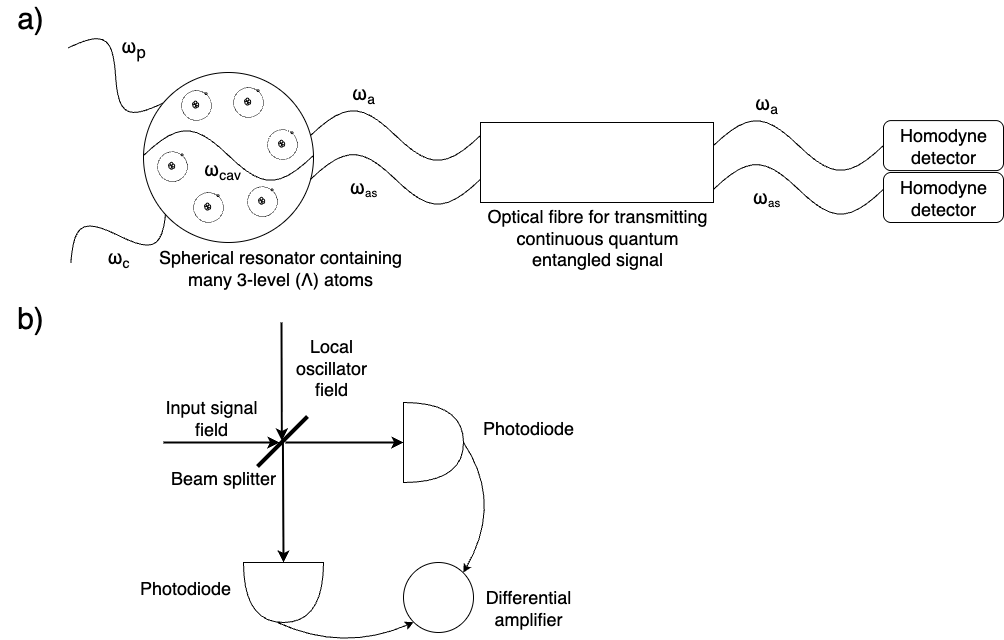
\includegraphics[width=\columnwidth]{SphericalResonatorAndHomodyne.png}
    \caption{Suggested setup of a real-world implementation for the four wave mixing process described with (a) two continuous beams entangled beams (continuous-variable entanglement) at frequencies $\omega_p$ and $\omega_c$ which undergo a four wave mixing process within a spherical resonator tuned to frequency $\omega_{cav}$ filled with cooled three-level atoms to produce Stokes and Anti-Stokes beams at frequencies $\omega_a$ and $\omega_{as}$, respectively. The resulting beams are then may then be sent through an optical fibre to homodyne detectors. (b) Homodyne detector layout.}
    \label{SphericalResonator}
\end{figure}

The outline of this project can be described in three stages: formulating up the system Hamiltonian, computationally solving for energy eigenstates of the Hamiltonian, and analyzing the results to find how changing specific parameters may change the system behavior.


\section{Background Information}

\subsection{Optical Non-Linearities}

\subsection{Electromagnetically Induced Transparency}

\subsection{Squeezed States}

\subsection{Three-Level Atom}

\begin{figure}
    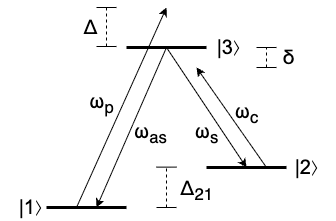
\includegraphics[width=\columnwidth]{ThreeLevelAtom.png}
    \caption{\textcolor{red}{TODO}}
    \label{ThreeLevelAtom}
\end{figure}

\subsection{Four Wave Mixing}

\subsection{Continuous Variable Entanglement}

\subsection{Fock Basis}

\subsection{Master Equation}




\section{Hamiltonian Formulation}


\section{Computational Methods}


\section{Results}


\section{Discussion}

\subsection{Conditions for Optical Squeezing}


\bibliography{refs}


\end{document}